\chapter{TenderInsights}

\section{Kurze Projektbeschreibung}
In dem Projekt geht es darum einen PoC - also einen Proof of Concept zu erstellen, der mithilfe von AI bzw. Large Language 
Models (LLM) große Dokumente nach gesuchten Inhalten durchsucht und aufbereitet. Im Fokus stehen dabei insbesondere 
öffentliche Ausschreibungen zur Akquise von neuen Projekten für das Unternehmen. Bisher hat ein Mitarbeiter aus PMO die 
Ausschreibungen händisch grob für passend oder nicht geeignet erklärt und diese dann an die Akquise weitergeleitet. 
Dort hat ein Mitarbeiter die Ausschreibung sehr genau analysiert und einen sogenannten One Pager erstellt, der alle 
Daten welche für eine Entscheidung, ob man sich bewerben möchte oder nicht, relevant sind. Aufgabe des PoC ist es nun 
diesen One Pager mithilfe von künstlicher Intelligenz und einem LLM aus einer oder mehreren bereitgestellten PDF-Datei zu 
generieren. Der Anwender soll dies über ein Userinterface im Stile einer Webanwendung bedienen können.

\section{Verwendete Software und Grundlagen}
In diesem Kapitel werden alle Software-Werkzeuge, Technologien und Begriffe beschrieben, welche im Entwicklungsumfeld des 
TenderInsights verwendet werden oder für ein Verständnis zuträglich sind.


\subsection{Technologien}
Bei der Entwicklung des TenderInsights werden viele unterschiedliche Technologien eingesetzt. Während meines Praktikums habe ich 
in meiner Tätigkeit als Entwickler viele davon kennengelernt und verwendet. Nachfolgend erkläre ich die wichtigsten Technologien.

\subsubsection{Python}
Python ist eine höhere Programmiersprache welche sich durch ihre klare und leicht verständliche Syntax auszeichnet.
Sie ist bekannt für ihre zahlreichen Standardbibliotheken und ihrer reichen Auswahl an Modulen und Frameworks.
Da OpenAI nur JavaScript und Python unterstützt, und Python aus zuvor genannten Gründen einsteigefreundlicher ist wurde sich 
für diese Sprache entschieden.

\subsubsection{Langchain}
Langchain ist ein Open-Source-Framework, das auf die Entwicklung und integration von Sprach-KI-Anwendungen spezialisiert ist.
Es erleichtert das einbinden von Sprachmodellen wie GPT-3.5-turbo von openAI in Projekte und wird beim TenderInsights für 
Textgenerierung verwendet.

\subsubsection{OpenAI - GPT}
OpenAI ist ein US-Amerikanisches Unternehmen welches sich mit der Erforschung und Entwicklung von künstlicher Intelligenz beschäftigt.
Eines der bekanntesten Tools bzw. Frameworks ist GPT - Generative Pretrained Transformer, ein Sprachverarbeitungsmodell zur Textgenerierung, 
Übersetzung, Zusammenfassung und mehr. GPT wird im TenderInsights verwendet um Information aus Texten zu extrahieren und um die 
gelieferten Prompts zu bewerten.

\subsubsection{Azure}
Microsoft Azure ist eine Cloud-Computing-Plattform, welche eine breite Palette von Diensten und Lösungen für Unternehmen und Entwickler bietet.
Zu den Entwickler-Tools und -Diensten gehört unter anderem Azure openAI, welches eine openAI API zur Verfügung stellt. Im Gegensatz zu openAI 
befinden sich die Server in Europa, weshalb im späteren Verlauf des Projekts aus Gründen des Datenschutzes zu Azure gewechselt wurde.

\subsubsection{ChromaDB}
ChromaDB ist eine Open-Source-Datenbanklösung, welche speziell für die Arbeit mit Vektor-Einbettungen in KI-Anwendungen entwickelt wurde.
Da der Kontext für Sprachmodelle stark unter der Größe von durchschnittlichen Dokumenten liegt wird eine Vektor-Datenbank genutzt um die relevanten
Stellen in den Dokumenten zu finden und als Kontext mit dem Prompt an das Sprachmodell für die Textgenerierung zu übergeben.

\subsubsection{JSON}
JavaScript Object Notation, oder kurz JSON, ist ein Daten-Austauschformat welches häufig verendet wird um Daten zwischen einem Server und einer 
Webanwendung zu übertragen. Da es für Menschen gut lesbar und für Maschinen einfach zu parsen (Entspricht einem normalen Dictionary in Python) 
ist eignet es sich hervorragend für das Speichern der OnePager Informationen.


\subsection{Werkzeuge}

\subsubsection{Visual Studio Code}
Visual Studio Code (VSCode) ist ein leistungsfähiger und anpassbarer Quelltext-Editor von Microsoft, der eine breite Palette von 
Programmiersprachen unterstützt und zahlreiche Erweiterungen für Entwickler bietet. 

\subsubsection{GitLab}
GitLab ist eine auf Git basierende webbasierte DevOps-Plattform, welche für die Versionskontrolle und CI/CD bei der Softwareentwicklung verwendet wird.

\subsubsection{Microsoft Teams}
Ein Kommunikationstool von Microsoft, welches genutzt wird um sich mit Kollegen auszutauschen, Dateien zu teilen und Besprechungen zu planen so wie durchzuführen.

\subsubsection{Jira}
Ein Projektmanagement-Werkzeug von Atlassian, das speziell für Softwareentwicklungsteams konzipiert ist und Funktionen für die Verfolgung von Aufgaben, Bugs und agile Prozesse bietet.
Es kam insbesondere beim verwalten des Backlogs und beim bearbeiten von Tickets zum Einsatz.

\subsubsection{Miro}
Eine digitale, kollaborative Whiteboard-Plattform, die es unserem Team ermöglicht, visuell zu brainstormen, zu planen und Projekte in Echtzeit zu gestalten.

\subsection{Wichtige Begriffe}

\begin{table}[H]
    \centering
    \caption{Wichtige Begriffe}
    \label{tab:technologien}
    \begin{tabular}{|l|l|}
    \hline
    \textbf{Name} & \textbf{Beschreibung} \\ \hline
    Prompt & Anleitung oder Frage die dem Sprachmodell vorgibt, was es tun soll \\ \hline
    Embedding & Einbetten von Text in Vektoren \\ \hline
    Name3 & Beschreibung3 \\ \hline
    \end{tabular}
\end{table}



\section{Projektstand bei Arbeitsbeginn}
Zum Zeitpunkt meines Projekteintrittes gibt es bereits ein Frontend welches mithilfe von Streamlit implementiert wurde. 
PDF-Dateien können über einen File-Uploader im Frontend an die Anwendung übergeben werden. Da die meisten LLM-Modelle eine 
begrenzte Token-Anzahl für die Abfragen haben ist es nicht möglich das gesamte Dokument an das LLM zu übergeben. 
Daher wird das Dokument aufgesplittet und mittels einer Vektordatenbank auf Ähnlichkeit mit die gesuchte Information 
abgeglichen. Die k Ergebnisse mit der größten Ähnlichkeit werden zusammen mit dem Prompt als Abfrage an das LLM übermittelt. 
Die Abfragen werden mit der Langchain API durchgführt, das verwendete Modell ist "gpt-3.5 turbo". Es gibt 3 Ausschreibungsdokumente 
in verschiedenen Größen mit denen die Abfragen getestet werden können. Es gibt 3 Prompts, welche bislang nur bedingt gute 
Ergebnisse liefern.

\section{Meine Rolle und Aufgaben im Projekt}
Ich bin in der Rolle eines Softwareentwickler in das Projekt gekommen. Meine Aufgabe bestand Anfangs darin, die Prompts für die einzelnen 
Felder des One Pagers zu formulieren um die gelieferten Ergebnisse zu verbessern. Dies resultierte in den Aufbau einer 
Test- und Evaluierungsarchitektur in Python mithilfe derer die Prompts vollautomatisch bewertet werden und anhand ihrer Kennzahl 
ausgewählt und weiter optimiert werden. Durch die Komplikationen mit dem Datenschutz wurde der Umstieg von Langchain auf 
Azure von Microsoft beschlossen, welchen ich durchgeführt habe. 

\subsection{Prompt Engineering}
Um gute Ergebnisse durch die Textvervollständigung der Sprachmodelle zu erhalten ist es unumgänglich hochwertige Prompts zu formulieren.
Hierfür habe ich mehrere E-Learnings zum Thema Prompt Engineering absolviert, in denen erklärt wird wie man hochwertige Prompts erstellt und 
ganze Systeme mit einer Chatbotintegration entwickelt. Besondere Methoden welche im Projekt zum Einsatz kommen sind Single-Shot-Prompting, 
bei dem man ein Beispiel gibt wie eine optimale Antwort auszusehen hat, und die Ausgabe als JSON festzulegen, um die erhaltenen Ergebnisse 
im Code nutzen und anwenden zu können. Das Bewerten der generierten Antworten durch das Sprachmodell um die Qualität zu messen, welches später 
im Kapitel \ref{chap:Evaluation} Verwendung findet.

\subsection{OnePager}
Der von PMO erstellte OnePager umfasst alle wesentlichen Information der Ausschreibung um eine fundierte Entscheidung darüber treffen zu 
können, ob die Ausschreibung als Projekt für iteratec geeignet ist. Informationen sind unter anderem der Projekttitel, eine kurze Projektbeschreibung, 
Adressdaten über das Ausschreibende Unternehmen oder Amt, wichtige Termine und Deadlines, Bewertungskriterien, Aufgaben und benötigte Unterlagen welche 
dem Angebot beigefügt werden müssen. Da jede dieser Punkte in unterschiedlichen Regionen der Dokumente zu finden ist und die Qualität der Ergebnisse 
besser ist wenn man nicht mehrere Fragen in einer Anfrage bündelt wird der OnePager in der Anwendung Frage für Frage zusammengesetzt und ergänzt.
Als Format wird JSON verwendet um später den fertigen OnePager gut speichern und weiterverarbeiten zu können (zum Beispiel für die Evaluation) und um dem
Frontend die Daten als Variable zur Verfügung zu stellen. Die OnePager-Klasse wurde wurde um viele Hilfsmethoden ausgestattet um das Arbeiten mit den 
JSON-Objekten zu erleichtert. Zu den Hilfsmethoden gehören unter anderem das initialisieren des OnePager-Template, das laden und abspeichern als Datei, 
einfaches hinzufügen von Teilinformationen aus den einzelnen Ergebnissen des Sprachmodells in den bestehenden OnePager und Prüffunktionen um nicht 
JSON-Konforme Antworten zu erkennen. 

\subsection{Evaluation}
\label{chap:Evaluation}

\subsection{Azure Migration}

\subsection{Messestand auf der BUILD23}

Zum Abschluss des Projektes wurden wir angefragt, ob wir 
aufgrund des hohen Interesses an dem Projekt eine Präsentation während des GS-Meetings und der BUILD23 halten möchten. 
Das erstellen der Präsentation und Vortragen dieser gehörte auch zu meinem Aufgabenbereich.

\section{Softwarearchitektur der Anwendung}

\begin{figure}[h]
    \centering
    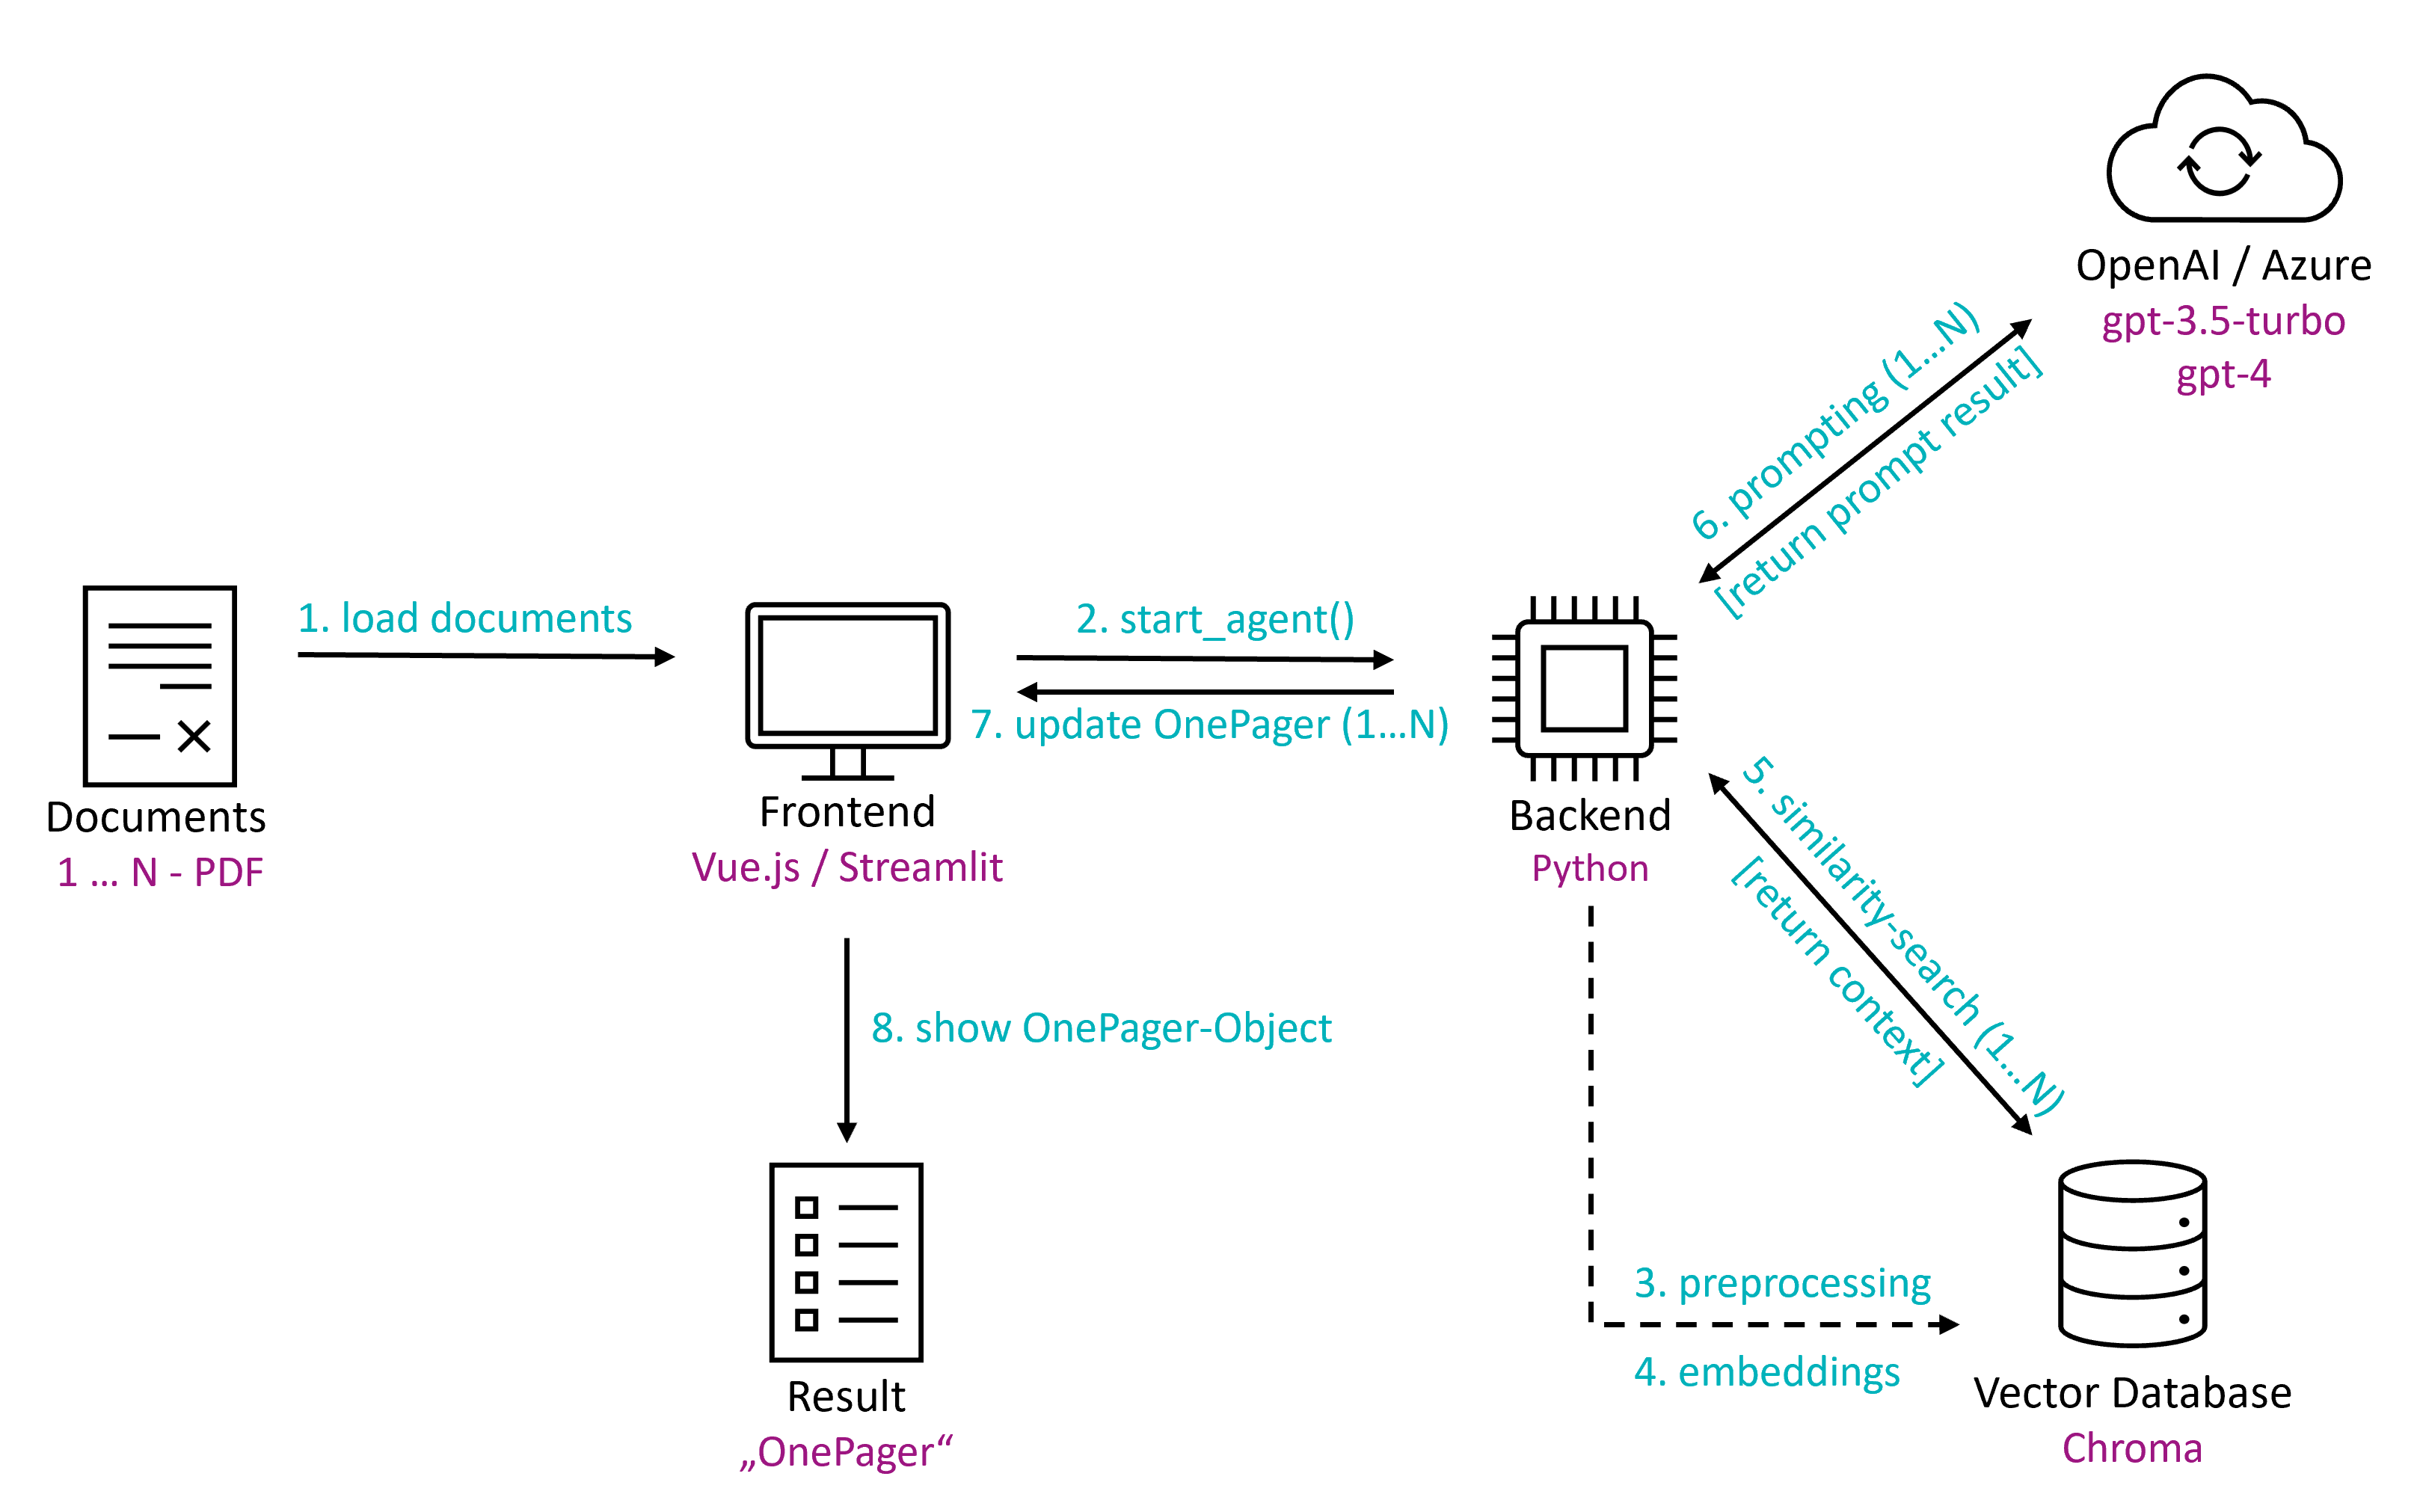
\includegraphics[width=0.8\textwidth]{figures/DokumentenAgent-Uebersicht.png}
    \caption{Schematische Darstellung der Software-Architektur}
    \label{fig:DokumentenAgent-uebersicht}    % \ref{fig:DokumentenAgent-uebersich}
\end{figure}

Anf: Datenschutz, große seiten, chatten mit Dokument
Grundlagen: Token, Similarity Search, Prompts

\section{Herausforderungen und Lösungsansätze}

\subsection{Optimierung der Prompts}
Um die Prompts zu verbessern ist es notwendig, diese an unterschiedlichen Ausschreibungen zu testen und das gelieferte 
Ergebnis mit der richtigen Antwort zu vergleichen. Da das größte Dokument über 100 Seiten hat und wir keine Musterlösungen 
haben war es schwierig Aussagen über die Qualität der Prompts zu treffen. Die Lösung war das Einführen einer Metrik welche 
die Qualität der Prompts misst. Es wurden 10 Dokumente ausgearbeitet und sämtliche wichtige Informationen in OnePager-JSON Dateien 
gespeichert. Anschließend wurde eine Testarchitektur geschaffen, in welcher man die gewünschten Prompts vollautomatisiert 
gegen die 10 Testdokumente abfragt und anschließend die Resultate zusammen mit der Musterlösung von ChatGPT auf inhaltliche 
Übereinstimmung überprüfen und bewerten lässt. Aus den so generierten Bewertungen lassen sich nun Aussagekräftige Kennzahlen 
generieren. Zur Darstellung wurde eine Visualisierungsklasse geschrieben, welche die Punktzahl der Prompts graphisch darstellt 
(siehe \ref{fig:03_Prompt_Evaluierung}) und so schnell erkennbar ist, ob der aktuelle Prompt zu einer Verbesserung 
oder Verschlechterung der Ergebnisse führt.

\begin{figure}[H]
    \centering
    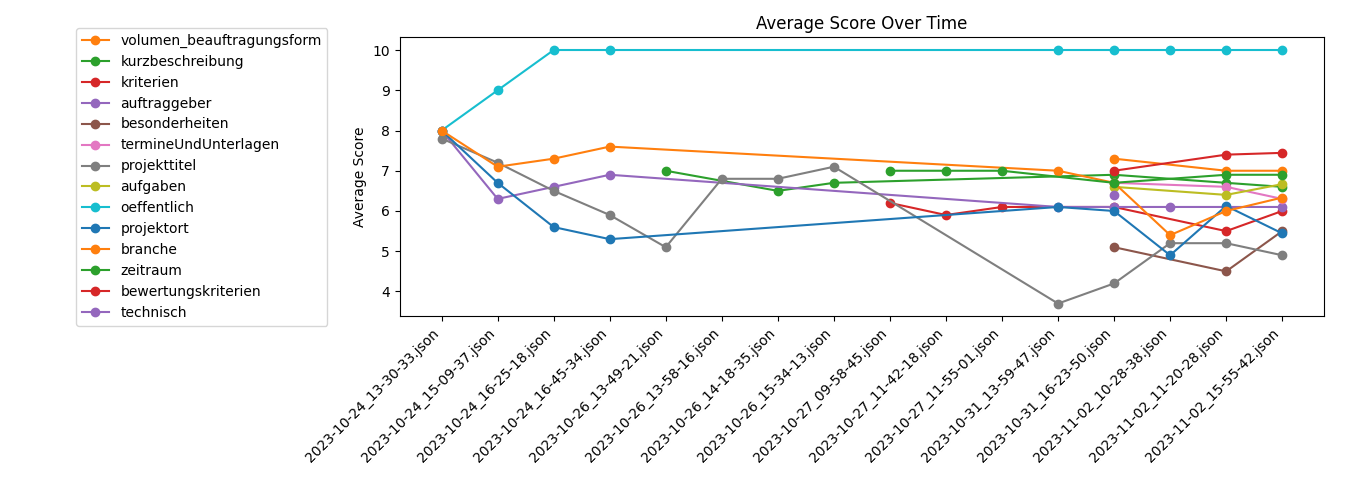
\includegraphics[width=0.8\textwidth]{figures/03_Prompt_Evaluierung.png}
    \caption{Visualisierung der durchschnittlichen Promptqualität im Laufe der Zeit}
    \label{fig:03_Prompt_Evaluierung}    % \ref{fig:03_Prompt_Evaluierung}
    \end{figure}

\subsection{Datenschutz}
Das übermitteln und verarbeiten von Personenbezogenen Daten ist in Deutschland nur mit Ausdrücklicher Genehmigung der 
entsprechenden Person zulässig. Es ist unklar inwiefern das Übermitteln der Daten aus den Dokumenten über die openAI 
API hierunter einzustufen ist. Offiziell heißt es, dass die Daten, welche über die API geteilt werden, nicht zu 
Trainingszwecken genutzt werden. Da die Server von openAI allerdings in den USA liegen gestalten sich Probleme mit 
europäischen Datenschutzrecht. Als Lösung wurde die Umstellung auf Azure in Betracht gezogen, da die Server auf europäischen 
Boden stehen und damit zumindest nach europäischen Recht Datenschutzkonform sind. Ein großer Nachteil von Azure ist aber, 
dass man für das erstellen der Vektordatenbank auf 16 Inputs beschränkt ist, während openAI hier keine Einschränkungen vorgibt. 
Größere Dokumente können leicht auf 1 Input pro Seite kommen, was ein Einbetten von Dokumenten ab 20 Seiten verhindert.
Um das Problem zu lösen habe ich statt die vorgegebene Embedding-Methode zu verwenden eine eigene Methode erstellt, 
welche die Dokumente bzw. die Inputs auf mehrere Listen mit einer Größe kleiner gleich 16 aufteilt. Anschließend werden 
die einzelnen Listen über eine REST API zu embeddings umgewandelt und anschließend wieder zusammengesetzt. Am ende wird eine 
Collection mit den Embeddings, den Dokumenten und entsprechenden Metadaten erstellt, welche zentral in einem VectorDataManager 
zur Verfügung gestellt wird. Gegen diese Collection können anschließend Abfragen wie Similarity-Searches durchgeführt werden.
Zusätzlich anonymisieren wir so gut wie alle Personenbezogenen Daten bevor wir diese an das Sprachmodell übermitteln, indem 
wir den Kontext vor dem Abschicken gegen eine Liste an Namen prüfen, und so Namen und Mailadressen herausfiltern.

\section{Ergebnisse und Erfahrungen}